% ============================================================
% S2 导学件量产·批6（轮4 最后一批）—— 章末「本章总结提升」板块（导学件线）
% 轮4 成卷·S2｜2026-09-12｜生成链：xelatex main.tex（两遍）→ python render.py（150dpi → png/pageN.png）
%
% 模板承 v11 样张族 `工作区/字替对照-0909/靠齐样张-0910/导学增量/` 章末页形制：
%   qp-fonts/qp-layout/qp-parts/qp-headfoot/qp-titles/qp-blocks 六宏＝课时02 原样拷贝（L1 冻结参数零改动）；
%   章末题头 \zhangmohead／题型标题 \lxing／类型总述 \zongshu／书写占位 \zhankong 等局部宏照抄样张；
%   \gaokaowei 空槽宏本件未用（高考题组＝独立板块定案，见 批6值台账）。
% 结构＝题型归类（12 型：类型总述两句式＋例＋变式）→ 精选高考题组（4 题，带 F6 源图）→ 知识脉络（全章结构文本树）。
%
% 取材链登记（详见 成卷/导学件/批6值台账.md）：
%   ① 12 型 24 题（例＋变式）＋高考组 4 题＝28 题全部取自 成卷/题面库/课时01~10 正文题，零新造；
%      与 10 课时导学件课中用题零同文（grep 断言复核，4 处假阳性已排除）；型名＝组名候选（待立组轮正名）。
%   ② 灯串＝难度(节号)口径（章末页无知识点块，登记口径）。
%   ③ 高考组真题元数据（年份/卷别）全章无源可考＝0 标注（G1 回填债随答案册轮）；F6 源图四件解包自
%      组卷网《空间向量与立体几何中的高考新题型》docx（映射取证 f6-annot.txt）。
%   ④ 清稿性修复（改字不改果）：L06Q16/L08Q6/L09Q7 题首「如图（所示），」删语（有言无图）；
%      L04Q14 题末补「（注：论断②不能作条件也不能作结论。）」（题面库清稿注义务）；
%      L04Q8 题末补填空线；半角标点→全角归一。
%   ⑤ 知识脉络树节名＝时间线基准表口径（1.1 三节＋1.2 五节）；全品原章末脉络图不在手，文本树代偿登记。
% 编译门：三 0（error＝0／Overfull＝0／Missing character＝0）。
% ============================================================
\documentclass[fontset=none]{ctexart}
\usepackage{qp-m3} % 换装：六宏→qp-m3 单包（钉后版 md5 7c3930362be8a0a2bdf21bbf8ac16573，两补钉随版）

% 局部字符类声明（本件限定，不动公共模块）：制表符段（U+2500–257F）改归 CJK 字类，
% 令知识脉络文本树的 ┣┃┗ 走中文字体（方正书宋_GBK 含 GB2312 第02区制表符），避免落西文缺字形。
\xeCJKDeclareCharClass{CJK}{"2500 -> "257F}

% ================= 页脚参数宏（qp-headfoot 文件头明示的复用入口，非模块语义改动） =================
\renewcommand{\qpzhangming}{第一章\quad 空间向量与立体几何}
\renewcommand{\qpjianming}{导学件}
\renewcommand{\qpceming}{高中数学\quad 选择性必修第一册(人教B版)} % 换装回钉：qp-m3 默认册名＝选必二，防页脚漂移（试迁规约）
% 册名沿用模块默认（qp-headfoot.tex＝人教B版）——2026-09-12 主脑勘正：本件属人教B版选必1，撤销批6 误换的 A 版行（原行 \renewcommand{\qpceming}{...(人教A版)} 已删）

% ================= 局部宏（照抄 v11 导学增量/main.tex 冻结定义；不动公共模块） =================
% 章末题头：章名 20.67pt \heizhang 左对齐（ZS-02 档）＋通栏 0.2pt 线（ZS-03）；
% 件型名「本章总结提升」走 \jietitle（16.88pt \hejie 居中＝ZS-04 档）。
\newcommand{\zhangmohead}[1]{%
  \par\addvspace{2pt}\noindent
  {\fontsize{20.67pt}{30pt}\selectfont\heizhang #1}\par
  \vspace{-0.3mm}\noindent\rule{\textwidth}{0.2pt}\par}
% 题型标题（TB-01 ◆标题件参数：12.03pt \heibf 2.3×＋◆ 0.63em＋后隙 2.4mm；前距 6.3pt／尾距 2pt 同 \zsd）
\newcommand{\lxing}[2]{\par\addvspace{6.3pt}\glueguard{4}%
  \noindent{\fontsize{12.03pt}{17pt}\selectfont\heibf \huafu\hspace{2.4mm}题型#1\quad #2}\par\addvspace{2pt}}
% 类型总述（XB-03 编注件式：半角 [ ] 标签＋正文级同号纯黑随文；两句式＝①识别信号＋②通法步骤）
\newcommand{\zongshu}[1]{\par\glueguard{1}\addvspace{2pt}%
  \noindent\anlabel{[类型总述]}\hspace{0.5em}#1\par\addvspace{2pt}}
% 纯书写占位留白（无水印；例→变式之间与变式后的书写位用）
% 局部宏 \zhankong 已由 qp-m3 收编（等值定义），依换装方案§1.4 预删防撞名

\begin{document}
%成书重装五本跨本连续页码（G7方案B，承M2/M3装配先例）setcounter 注入位
\setcounter{page}{35}

% ============================================================
% 章末「本章总结提升」：题型归类（12 型）→ 精选高考题组（4 题）→ 知识脉络
% ============================================================
\zhangmohead{第一章\quad 空间向量与立体几何}
\jietitle{本章总结提升}

\begin{multicols}{2}
\emergencystretch=1em

\huaxing{题}{型}{归}{类}{通法提炼\quad 例变对接}

% ---------- 题型一：概念与线性运算化简（例＝课时02第1题 F2·1；变式＝课时02第2题 F2·4） ----------
\vbox{
\lxing{一}{概念与线性运算化简}

\zongshu{①识别：题干围绕空间向量的相等、平行、共面等概念罗列命题要求判断，或在多面体中要求向量线性运算的化简定向时，判归本题型.②通法：概念命题对照定义逐条核验，零向量与相反向量处备反例；化简按加减法则把向量首尾相接合并，再与目标向量逐一对验.}

\li{例\textbf{1}}{简单(1.1.1)}{下列关于空间向量的命题中，正确命题的个数是(\kongwei)}{}

\bindp {\fontsize{10.5pt}{19pt}\selectfont ①任一向量与它的相反向量都不相等；\par}

\bindp {\fontsize{10.5pt}{19pt}\selectfont ②长度相等、方向相同的两个向量是相等向量；\par}

\bindp {\fontsize{10.5pt}{19pt}\selectfont ③平行且模相等的两个向量是相等向量；\par}

\bindp {\fontsize{10.5pt}{19pt}\selectfont ④若\(\overrightarrow{a}\neq\overrightarrow{b}\)，则\(|\overrightarrow{a}|\neq|\overrightarrow{b}|\)；\par}

\bindp {\fontsize{10.5pt}{19pt}\selectfont ⑤两个向量相等，则它们的起点与终点相同.\par}

\bindopt {\fontsize{10.5pt}{19pt}\selectfont \makebox[\dimexpr0.25\linewidth-0.5em\relax][l]{A．\(0\)；}\makebox[\dimexpr0.25\linewidth-0.5em\relax][l]{B．\(1\)；}\makebox[\dimexpr0.25\linewidth-0.5em\relax][l]{C．\(2\)；}\makebox[\dimexpr0.25\linewidth-0.5em\relax][l]{D．\(3\)}\par}

\zhankong{13mm}

\begin{ansblock}[导-章末-例1]
% ans:导-章末-例1
\ansnote{例1}{B（仅②真）}
\end{ansblock}
\liB{变式\textbf{1}}{简单(1.1.1)}{在正方体\(ABCD\text{-}\penalty100 A_{1}B_{1}C_{1}D_{1}\)中，下列各式的运算结果为向量\(\overrightarrow{B_{1}D_{1}}\)的是(\kongwei)}{}

\bindp {\fontsize{10.5pt}{19pt}\selectfont ①\(\overrightarrow{A_{1}D_{1}}-\overrightarrow{A_{1}A}-\overrightarrow{AB}\)；\quad ②\(\overrightarrow{BC}+\overrightarrow{BB_{1}}-\overrightarrow{D_{1}C_{1}}\)；\par}

\bindp {\fontsize{10.5pt}{19pt}\selectfont ③\(\overrightarrow{AD}-\overrightarrow{AB_{1}}+\overrightarrow{DD_{1}}\)；\quad ④\(\overrightarrow{B_{1}D_{1}}-\overrightarrow{AA_{1}}+\overrightarrow{DD_{1}}\).\par}

\bindopt {\fontsize{10.5pt}{19pt}\selectfont \makebox[\dimexpr0.25\linewidth-0.5em\relax][l]{A．①②；}\makebox[\dimexpr0.25\linewidth-0.5em\relax][l]{B．②③；}\makebox[\dimexpr0.25\linewidth-0.5em\relax][l]{C．③④；}\makebox[\dimexpr0.25\linewidth-0.5em\relax][l]{D．①④}\par}

\zhankong{6mm}

\begin{ansblock}[导-章末-变式1]
% ans:导-章末-变式1
\ansnote{变式1}{C（③④）}
\end{ansblock}


% ---------- 题型二：数量积与模、夹角互求（例＝课时02第7题 1.1.1练习A·3；变式＝课时02第14题 习题1—1B·7） ----------
}

\vbox{
\lxing{二}{数量积与模、夹角互求}

\zongshu{①识别：题干给出模与夹角求数量积，或由数量积、模的等量关系反求两向量夹角时，判归本题型.②通法：紧扣定义\(\overrightarrow{a}\cdot\overrightarrow{b}=|\overrightarrow{a}||\overrightarrow{b}|\cos\langle\overrightarrow{a},\overrightarrow{b}\rangle\)与\(\overrightarrow{a}\cdot\overrightarrow{a}=|\overrightarrow{a}|^{2}\)双向转化；含模的条件先平方展开解出\(\cos\langle\overrightarrow{a},\overrightarrow{b}\rangle\)，再按夹角范围\([0,\pi]\)取角.}

\li{例\textbf{2}}{简单(1.1.1)}{已知\(ABCD\text{-}\penalty100 A_{1}B_{1}C_{1}D_{1}\)是一个正方体，写出下列向量夹角的大小：}{}

\bindp {\fontsize{10.5pt}{19pt}\selectfont (1)\(\langle\overrightarrow{AB},\overrightarrow{CC_{1}}\rangle\)；\qquad (2)\(\langle\overrightarrow{DD_{1}},\overrightarrow{BA_{1}}\rangle\).}

\zhankong{13mm}

\begin{ansblock}[导-章末-例2]
% ans:导-章末-例2
\ansnote{例2}{(1)\(90^{\circ}\)；(2)\(45^{\circ}\)}
\end{ansblock}
\liB{变式\textbf{2}}{简单(1.1.1)}{已知\(\overrightarrow{a},\overrightarrow{b}\)是非零空间向量，根据下列各条件分别求\(\langle\overrightarrow{a},\overrightarrow{b}\rangle\)：}{}

\bindp {\fontsize{10.5pt}{19pt}\selectfont (1)\(\overrightarrow{a}\cdot\overrightarrow{b}=-|\overrightarrow{a}||\overrightarrow{b}|\)；\quad (2)\(|\overrightarrow{a}|=|\overrightarrow{b}|=|\overrightarrow{a}-\overrightarrow{b}|\)；\par}

\bindp {\fontsize{10.5pt}{19pt}\selectfont (3)\(|\overrightarrow{a}|=|\overrightarrow{b}|=|\overrightarrow{a}+\overrightarrow{b}|\)；\quad (4)\(|\overrightarrow{a}+\overrightarrow{b}|=|\overrightarrow{a}-\overrightarrow{b}|\).}

\zhankong{6mm}

\begin{ansblock}[导-章末-变式2]
% ans:导-章末-变式2
\ansnote{变式2}{(1)\(\pi\)；(2)\(\dfrac{\pi}{3}\)；(3)\(\dfrac{2\pi}{3}\)；(4)\(\dfrac{\pi}{2}\)}
\end{ansblock}


% ---------- 题型三：数量积存在性判断与最值（例＝课时02第13题 F2·27；变式＝课时01第16题 复习题C·3） ----------
}

\vbox{
\lxing{三}{数量积存在性判断与最值}

\zongshu{①识别：题干问若干数量积能否为0(存在性判断)，或在动点背景下求数量积的最值时，判归本题型.②通法：存在性问题选基底或建系，把每个数量积表为棱长参数式，能取0即存在；动点最值题先用共线条件化简向量和，再建系配成关于动点坐标的二次式求最值.}

\li{例\textbf{3}\duoxuan}{中档(1.1.1)}{已知长方体\(ABCD\text{-}\penalty100 A_{1}B_{1}C_{1}D_{1}\)，则下列向量的数量积可以为0的是(\kongwei)}{}

\bindopt {\fontsize{10.5pt}{19pt}\selectfont \makebox[\dimexpr0.5\linewidth-1em\relax][l]{A．\(\overrightarrow{AD_{1}}\cdot\overrightarrow{B_{1}C}\)；}\makebox[\dimexpr0.5\linewidth-1em\relax][l]{B．\(\overrightarrow{BD_{1}}\cdot\overrightarrow{AC}\)；}\par}

\bindopt {\fontsize{10.5pt}{19pt}\selectfont \makebox[\dimexpr0.5\linewidth-1em\relax][l]{C．\(\overrightarrow{AB}\cdot\overrightarrow{AD_{1}}\)；}\makebox[\dimexpr0.5\linewidth-1em\relax][l]{D．\(\overrightarrow{BD_{1}}\cdot\overrightarrow{BC}\)}\par}

\zhankong{13mm}

\begin{ansblock}[导-章末-例3]
% ans:导-章末-例3
\ansnote{例3}{ABC（\(D\) 支 \(D=b^{2}\) 恒正）}
\end{ansblock}
\liB{变式\textbf{3}}{难(1.1.1)}{已知\(\triangle ABC\)是边长为2的等边三角形，\(P\)为平面\(ABC\)内的一点，求\nobreak\(\overrightarrow{PA}\cdot(\overrightarrow{PB}+\overrightarrow{PC})\)的最小值.}{}

\zhankong{6mm}

\begin{ansblock}[导-章末-变式3]
% ans:导-章末-变式3
\ansnote{变式3}{最小值 \(-\dfrac{3}{2}\)；\(P\) 为高线 \(AM\) 中点（\(M\) 为 \(BC\) 中点）}
\end{ansblock}


% ---------- 题型四：基底判定与共面分解（例＝课时03第2题 F3·1；变式＝课时03第16题 习题1—1C·4） ----------
}

\vbox{
\lxing{四}{基底判定与共面分解}

\zongshu{①识别：题干判断三个向量能否构成空间基底，或要求以基底分解向量、证明点共面时，判归本题型.②通法：基底判定归结为检验三向量是否共面(不能共面即可)；分解时选定不共面基底，用线性运算把目标向量逐层展开；四点共面用共面向量定理或“系数和＝1”判据.}

\li{例\textbf{4}}{简单(1.1.2)}{在以下三个命题中，真命题的个数是(\kongwei)}{}

\bindp {\fontsize{10.5pt}{19pt}\selectfont ①若三个非零向量\(\overrightarrow{a},\overrightarrow{b},\overrightarrow{c}\)不能构成空间的一个基底，则\(\overrightarrow{a},\overrightarrow{b},\overrightarrow{c}\)共面；\par}

\bindp {\fontsize{10.5pt}{19pt}\selectfont ②若两个非零向量\(\overrightarrow{a},\overrightarrow{b}\)与任何一个向量都不能构成空间的一个基底，则\(\overrightarrow{a},\overrightarrow{b}\)共线；\par}

\bindp {\fontsize{10.5pt}{19pt}\selectfont ③若\(\overrightarrow{a},\overrightarrow{b}\)是两个不共线的向量，而\(\overrightarrow{c}=\lambda\overrightarrow{a}+\mu\overrightarrow{b}(\lambda,\mu\in\mathbf{R}\)且\(\lambda\mu\neq0)\)，则\(\{\overrightarrow{a},\overrightarrow{b},\overrightarrow{c}\}\)构成空间的一个基底.\par}

\bindopt {\fontsize{10.5pt}{19pt}\selectfont \makebox[\dimexpr0.25\linewidth-0.5em\relax][l]{A．\(0\)；}\makebox[\dimexpr0.25\linewidth-0.5em\relax][l]{B．\(1\)；}\makebox[\dimexpr0.25\linewidth-0.5em\relax][l]{C．\(2\)；}\makebox[\dimexpr0.25\linewidth-0.5em\relax][l]{D．\(3\)}\par}

\zhankong{13mm}

\begin{ansblock}[导-章末-例4]
% ans:导-章末-例4
\ansnote{例4}{C（①②真③假）}
\end{ansblock}
\liB{变式\textbf{4}}{难(1.1.2)}{已知\(A,B,C\)是空间中不共线的三点，\(O\)是空间中任意一点.求证：\(P\)在平面\(ABC\)内的充要条件是，存在满足\(x+y+z=1\)的实数\(x,y,z\)，使得\nobreak\(\overrightarrow{OP}=x\overrightarrow{OA}+y\overrightarrow{OB}+z\overrightarrow{OC}\).}{}

\zhankong{6mm}

\begin{ansblock}[导-章末-变式4]
% ans:导-章末-变式4
\ansnote{变式4}{证明见解析}
\end{ansblock}


% ---------- 题型五：建系与坐标表示（例＝课时04第8题 习题1—1A·7；变式＝课时04第13题 习题1—1B·5） ----------
}

\vbox{
\lxing{五}{建系与坐标表示}

\zongshu{①识别：题干要求建立空间直角坐标系表示点与向量的坐标，或辨析点的对称坐标时，判归本题型.②通法：过同一顶点选两两垂直的三条棱作坐标轴，按棱长沿轴定位写坐标；对称关系按“关于谁不变谁、其余变号”逐条检验；平行六面体抓住对角线交点的中心对称求顶点坐标.}

\li{例\textbf{5}}{简单(1.1.3)}{在空间直角坐标系中，已知点\(P(x,y,z)\)，下列叙述正确的序号有\kongbai{}.}{}

\bindp {\fontsize{10.5pt}{19pt}\selectfont ①点\(P\)关于\(x\)轴的对称点是\(P_{1}(x,-y,z)\)；\par}

\bindp {\fontsize{10.5pt}{19pt}\selectfont ②点\(P\)关于\(yOz\)平面的对称点是\(P_{2}(x,-y,-z)\)；\par}

\bindp {\fontsize{10.5pt}{19pt}\selectfont ③点\(P\)关于\(y\)轴的对称点是\(P_{3}(x,-y,z)\)；\par}

\bindp {\fontsize{10.5pt}{19pt}\selectfont ④点\(P\)关于原点的对称点是\(P_{4}(-x,-y,-z)\).\par}

\zhankong{13mm}

\begin{ansblock}[导-章末-例5]
% ans:导-章末-例5
\ansnote{例5}{④（逐条对称律验）}
\end{ansblock}
\liB{变式\textbf{5}}{中档(1.1.3)}{已知空间直角坐标系中，平行六面体\(ABCD\text{-}\penalty100 A_{1}B_{1}C_{1}D_{1}\)满足：\(A(-2,1,3)\)，\(B(2,2,1)\)，\(C(3,4,2)\)，\(D(-1,3,4)\)，且平行六面体的体对角线的交点为\(M(1,1,1)\)，求\(A_{1},B_{1},C_{1},D_{1}\)的坐标.}{}

\zhankong{6mm}

\begin{ansblock}[导-章末-变式5]
% ans:导-章末-变式5
\ansnote{变式5}{\(A_{1}(-1,-2,0)\)，\(B_{1}(3,-1,-2)\)，\(C_{1}(4,1,-1)\)，\(D_{1}(0,0,1)\)}
\end{ansblock}


% ---------- 题型六：坐标公式·夹角·投影链（例＝课时05第8题 1.1.3练习B·3；变式＝课时05第11题 T4） ----------
}

\vbox{
\lxing{六}{坐标公式·夹角·投影链}

\zongshu{①识别：题干在坐标表示下求向量夹角、线段长、投影数量或反求参数时，判归本题型.②通法：套用坐标公式链——模\(|\overrightarrow{a}|=\sqrt{x^{2}+y^{2}+z^{2}}\)、夹角余弦\(\cos\langle\overrightarrow{a},\overrightarrow{b}\rangle=\frac{\overrightarrow{a}\cdot\overrightarrow{b}}{|\overrightarrow{a}||\overrightarrow{b}|}\)、投影数量\(\frac{\overrightarrow{a}\cdot\overrightarrow{b}}{|\overrightarrow{b}|}\)；多问链题以前问结果作后问数据，逐问推进.}

\li{例\textbf{6}}{简单(1.1.3)}{求下列两个空间向量夹角的余弦：}{}

\bindp {\fontsize{10.5pt}{19pt}\selectfont (1)\(\overrightarrow{a}=(2,-3,\sqrt{3})\)，\(\overrightarrow{b}=(1,0,0)\)；\qquad (2)\(\overrightarrow{a}=(-1,-1,1)\)，\(\overrightarrow{b}=(-1,0,1)\).}

\zhankong{13mm}

\begin{ansblock}[导-章末-例6]
% ans:导-章末-例6
\ansnote{例6}{(1)\(\dfrac{1}{2}\)；(2)\(\dfrac{\sqrt{6}}{3}\)}
\end{ansblock}
\liB{变式\textbf{6}}{中档(1.1.3)}{已知点\(A(0,1,2)\)，\(B(1,-1,3)\)，\(C(1,5,-1)\).}{}

\bindp {\fontsize{10.5pt}{19pt}\selectfont (1)若\(D\)为线段\(BC\)的中点，求线段\(AD\)的长；\par}

\bindp {\fontsize{10.5pt}{19pt}\selectfont (2)若\(\overrightarrow{AD}=(2,a,1)\)，且\(\overrightarrow{AB}\cdot\overrightarrow{AD}=1\)，求\(a\)的值，并求此时向量\(\overrightarrow{AB}\)与\(\overrightarrow{AD}\)夹角的余弦值.}

\zhankong{6mm}

\begin{ansblock}[导-章末-变式6]
% ans:导-章末-变式6
\ansnote{变式6}{(1)\(\sqrt{3}\)；(2)\(a=1\)，\(\cos=\dfrac{1}{6}\)}
\end{ansblock}


% ---------- 题型七：平行垂直坐标条件求参（例＝课时05第6题 E12；变式＝课时05第7题 E14） ----------
}

\vbox{
\lxing{七}{平行垂直坐标条件求参}

\zongshu{①识别：题干以坐标形式给出平行、垂直或模长条件，反求向量中的参数时，判归本题型.②通法：平行\(\Leftrightarrow\)对应坐标成比例(或存在\(\lambda\)使\(\overrightarrow{a}=\lambda\overrightarrow{b}\))，垂直\(\Leftrightarrow\)数量积的坐标式为0，模长\(\Leftrightarrow\)坐标平方和开方；按条件列方程(组)解参数，多解时结合题意取舍.}

\li{例\textbf{7}}{简单(1.1.3)}{已知\(\overrightarrow{a}=(-2,3,2)\)，\(\overrightarrow{b}=(1,-5,1)\)，且\(m\overrightarrow{a}+\overrightarrow{b}\)与\(2\overrightarrow{a}-\overrightarrow{b}\)平行，求实数\(m\)的值.}{}

\zhankong{13mm}

\begin{ansblock}[导-章末-例7]
% ans:导-章末-例7
\ansnote{例7}{\(m=-2\)}
\end{ansblock}
\liB{变式\textbf{7}}{简单(1.1.3)}{向量\(\overrightarrow{a}=(2,1,x)\)，\(\overrightarrow{b}=(2,y,-1)\)，若\(|\overrightarrow{a}|=\sqrt{5}\)，且\(\overrightarrow{a}\perp\overrightarrow{b}\)，则\(x+y\)的值为(\kongwei)}{}

\bindopt {\fontsize{10.5pt}{19pt}\selectfont \makebox[\dimexpr0.25\linewidth-0.5em\relax][l]{A．\(-1\)；}\makebox[\dimexpr0.25\linewidth-0.5em\relax][l]{B．\(1\)；}\makebox[\dimexpr0.25\linewidth-0.5em\relax][l]{C．\(-4\)；}\makebox[\dimexpr0.25\linewidth-0.5em\relax][l]{D．\(4\)}\par}

\zhankong{6mm}

\begin{ansblock}[导-章末-变式7]
% ans:导-章末-变式7
\ansnote{变式7}{C（\(x+y=-4\)）}
\end{ansblock}


% ---------- 题型八：方向向量与线线位置（例＝课时06第4题 F5·4；变式＝课时06第16题 1.2.1练习B·4〔图删语清稿〕） ----------
}

\vbox{
\lxing{八}{方向向量与线线位置}

\zongshu{①识别：题干借直线的方向向量判断两直线平行、垂直或求异面直线所成角，或探究两直线公垂线段上的点是否存在时，判归本题型.②通法：方向向量共线\(\Leftrightarrow\)两直线平行(须去重合)，数量积为0\(\Leftrightarrow\)两直线垂直；所成角用\(\cos\theta=|\cos\langle\overrightarrow{v_{1}},\overrightarrow{v_{2}}\rangle|\)锐角化；存在性问题建系设参数点，由两个垂直条件列方程组求解.}

\li{例\textbf{8}}{简单(1.2.1)}{\(l_{1}\)的方向向量为\(\overrightarrow{v_{1}}=(1,2,3)\)，\(l_{2}\)的方向向量\(\overrightarrow{v_{2}}=(\lambda,4,6)\)，若\(l_{1}\parallel l_{2}\)，则\(\lambda\)等于(\kongwei)}{}

\bindopt {\fontsize{10.5pt}{19pt}\selectfont \makebox[\dimexpr0.25\linewidth-0.5em\relax][l]{A．\(1\)；}\makebox[\dimexpr0.25\linewidth-0.5em\relax][l]{B．\(2\)；}\makebox[\dimexpr0.25\linewidth-0.5em\relax][l]{C．\(3\)；}\makebox[\dimexpr0.25\linewidth-0.5em\relax][l]{D．\(4\)}\par}

\zhankong{13mm}

\begin{ansblock}[导-章末-例8]
% ans:导-章末-例8
\ansnote{例8}{B（\(\lambda=2\)）}
\end{ansblock}
\liB{变式\textbf{8}}{难(1.2.1)}{已知长方体\(ABCD\text{-}\penalty100 A_{1}B_{1}C_{1}D_{1}\)中，\(AD=AB=2DD_{1}\)，判断满足下列条件的点\(M,N\)是否存在：\(M\in AD_{1}\)，\(N\in BD\)，\(MN\perp AD_{1}\)，\(MN\perp BD\).}{}

\zhankong{6mm}

\begin{ansblock}[导-章末-变式8]
% ans:导-章末-变式8
\ansnote{变式8}{存在；\(|MN|=\dfrac{\sqrt{6}}{3}\)}
\ansnote{解析}{\(D\) 原点系 \(D(0,0,0)\)，\(A(2,0,0)\)，\(B(2,2,0)\)，\(D_{1}(0,0,1)\)：\(M\left(\dfrac{2}{3},0,\dfrac{2}{3}\right)\)，\(N\left(\dfrac{1}{3},\dfrac{1}{3},0\right)\)。}
\end{ansblock}


% ---------- 题型九：法向量与平行垂直判定（例＝课时07第3题 池1.2.1.2-1；变式＝课时07第4题 F7·9） ----------
}

\vbox{
\lxing{九}{法向量与平行垂直判定}

\zongshu{①识别：题干给出(或需求)平面的法向量，据以判定或证明线面、面面的平行与垂直时，判归本题型.②通法：解方程组\(\overrightarrow{n}\cdot\overrightarrow{a}=0\)且\(\overrightarrow{n}\cdot\overrightarrow{b}=0\)求法向量；线面平行\(\Leftrightarrow\)\(\overrightarrow{v}\cdot\overrightarrow{n}=0\)且线在面外，线面垂直\(\Leftrightarrow\)\(\overrightarrow{v}\parallel\overrightarrow{n}\)，面面平行\(\Leftrightarrow\)两法向量共线，面面垂直\(\Leftrightarrow\)两法向量数量积为0.}

\li{例\textbf{9}}{简单(1.2.2)}{已知直线\(l\)的方向向量是\(\overrightarrow{a}=(3,2,1)\)，平面\(\alpha\)的法向量是\(\overrightarrow{u}=(-1,2,-1)\)，则\(l\)与\(\alpha\)的位置关系是(\kongwei)}{}

\bindopt {\fontsize{10.5pt}{19pt}\selectfont \makebox[\dimexpr0.5\linewidth-1em\relax][l]{A．\(l\perp\alpha\)；}\makebox[\dimexpr0.5\linewidth-1em\relax][l]{B．\(l\parallel\alpha\)；}\par}

\bindopt {\fontsize{10.5pt}{19pt}\selectfont C．\(l\)与\(\alpha\)相交但不垂直；\par}

\bindopt {\fontsize{10.5pt}{19pt}\selectfont D．\(l\parallel\alpha\)或\(l\subset\alpha\)\par}

\zhankong{13mm}

\begin{ansblock}[导-章末-例9]
% ans:导-章末-例9
\ansnote{例9}{D}
\end{ansblock}
\liB{变式\textbf{9}\duoxuan}{简单(1.2.2)}{下列命题是真命题的有(\kongwei)}{}

\bindp {\fontsize{10.5pt}{19pt}\selectfont A．直线\(l\)的方向向量为\(\overrightarrow{a}=(1,-1,2)\)，直线\(m\)的方向向量为\(\overrightarrow{b}=(2,1,-\frac{1}{2})\)，则\(l\)与\(m\)垂直；\par}

\bindp {\fontsize{10.5pt}{19pt}\selectfont B．直线\(l\)的方向向量为\(\overrightarrow{a}=(0,1,-1)\)，平面\(\alpha\)的法向量为\(\overrightarrow{n}=(1,-1,-1)\)，则\(l\perp\alpha\)；\par}

\bindp {\fontsize{10.5pt}{19pt}\selectfont C．平面\(\alpha,\beta\)的法向量分别为\(\overrightarrow{n_{1}}=(0,1,3)\)，\(\overrightarrow{n_{2}}=(1,0,2)\)，则\(\alpha\parallel\beta\)；\par}

\bindp {\fontsize{10.5pt}{19pt}\selectfont D．平面\(\alpha\)经过三点\(A(1,0,-1)\)，\(B(0,1,0)\)，\(C(-1,2,0)\)，向量\(\overrightarrow{n}=(1,u,t)\)是平面\(\alpha\)的法向量，则\(u+t=1\).\par}

\zhankong{6mm}

\begin{ansblock}[导-章末-变式9]
% ans:导-章末-变式9
\ansnote{变式9}{AD}
\end{ansblock}


% ---------- 题型十：线面角定义法与向量法（例＝课时08第1题 1.2.3练习A·2；变式＝课时08第6题 练习B·3〔图删语清稿〕） ----------
}

\vbox{
\lxing{十}{线面角定义法与向量法}

\zongshu{①识别：题干求直线与平面所成的角，或由线面角反求斜线段、射影的长时，判归本题型.②通法：定义法先找(作)斜线在平面内的射影，射影长＝斜线长\(\times\cos\theta\)；向量法求方向向量与法向量的夹角，用\(\sin\theta=|\cos\langle\overrightarrow{v},\overrightarrow{n}\rangle|\)得线面角.}

\li{例\textbf{10}}{简单(1.2.3)}{已知直线\(l\)与平面\(\alpha\)所成的角为\(\theta\)，且\(A,B\)是直线\(l\)上两点，分别根据以下条件，求线段\(AB\)在平面\(\alpha\)内的射影的长：}{}

\bindp {\fontsize{10.5pt}{19pt}\selectfont (1)\(AB=6\)，\(\theta=\frac{\pi}{6}\)；\qquad (2)\(AB=10\)，\(\theta=\frac{\pi}{4}\).}

\zhankong{13mm}

\begin{ansblock}[导-章末-例10]
% ans:导-章末-例10
\ansnote{例10}{(1)\(3\sqrt{3}\)；(2)\(5\sqrt{2}\)}
\end{ansblock}
\liB{变式\textbf{10}}{中档(1.2.3)}{已知正方体\(ABCD\text{-}\penalty100 A_{1}B_{1}C_{1}D_{1}\)中，\(M\)是\(BB_{1}\)的中点，求直线\(A_{1}M\)与平面\(AMC_{1}\)所成角的正弦值.}{}

\zhankong{6mm}

\begin{ansblock}[导-章末-变式10]
% ans:导-章末-变式10
\ansnote{变式10}{\(\dfrac{2\sqrt{30}}{15}\)}
\end{ansblock}


% ---------- 题型十一：二面角的求法（例＝课时09第1题 1.2.4练习A·1；变式＝课时09第7题 复习题C·4〔图删语清稿·亲算验证〕） ----------
}

\vbox{
\lxing{十一}{二面角的求法}

\zongshu{①识别：题干求二面角(的平面角或其余弦值)，或由二面角反求射影面积、点面距离时，判归本题型.②通法：定义法在棱上取点，在两个半平面内各作棱的垂线得平面角；向量法求两半平面法向量的夹角，再结合图形判断取锐角还是补角；射影型用\(S'=S\cos\theta\)求射影面积.}

\li{例\textbf{11}}{简单(1.2.4)}{已知二面角\(P\text{-}\penalty100 AB\text{-}\penalty100 P'\)的大小为\(\frac{\pi}{6}\)，且\(PP'\perp\)平面\(ABP'\)，\(\triangle ABP\)的面积为3，求\(\triangle ABP'\)的面积.}{}

\zhankong{13mm}

\begin{ansblock}[导-章末-例11]
% ans:导-章末-例11
\ansnote{例11}{\(\dfrac{3\sqrt{3}}{2}\)}
\end{ansblock}
\liB{变式\textbf{11}}{难(1.2.4)}{已知四棱锥\(P\text{-}\penalty100 ABCD\)中，\(PB\perp AD\)，侧面\(PAD\)为边长等于2的正三角形，底面\(ABCD\)为菱形，侧面\(PAD\)与底面\(ABCD\)所成的二面角为\(120^\circ\).}{}

\bindp {\fontsize{10.5pt}{19pt}\selectfont (1)求点\(P\)到平面\(ABCD\)的距离；\par}

\bindp {\fontsize{10.5pt}{19pt}\selectfont (2)求二面角\(A\text{-}\penalty100 PB\text{-}\penalty100 C\)的余弦值.}

\zhankong{6mm}

\begin{ansblock}[导-章末-变式11]
% ans:导-章末-变式11
\ansnote{变式11}{(1)\(\dfrac{3}{2}\)；(2)\(-\dfrac{2\sqrt{7}}{7}\)}
\end{ansblock}


% ---------- 题型十二：空间距离（例＝课时10第3题 F5·12；变式＝课时10第12题 F5·14） ----------
}

\vbox{
\lxing{十二}{空间距离}

\zongshu{①识别：题干求点到直线、点到平面的距离，或平行平面间、异面直线间的距离时，判归本题型.②通法：点面距\(d=\frac{|\overrightarrow{PA}\cdot\overrightarrow{n}|}{|\overrightarrow{n}|}\)；点线距把斜线段向直线方向向量分解，勾股链开方得\(d=\sqrt{|\overrightarrow{PA}|^{2}-|\overrightarrow{PA}\cdot\overrightarrow{e}|^{2}}\)(\(\overrightarrow{e}\)为单位方向向量)；线面距、面面距与异面直线距先转化为点面距.}

\li{例\textbf{12}}{简单(1.2.5)}{已知\(A(0,0,2)\)，\(B(1,0,2)\)，\(C(0,2,0)\)，则点\(A\)到直线\(BC\)的距离为(\kongwei)}{}

\bindopt {\fontsize{10.5pt}{19pt}\selectfont \makebox[\dimexpr0.25\linewidth-0.5em\relax][l]{A．\(\frac{2\sqrt{2}}{3}\)；}\makebox[\dimexpr0.25\linewidth-0.5em\relax][l]{B．\(1\)；}\makebox[\dimexpr0.25\linewidth-0.5em\relax][l]{C．\(\sqrt{2}\)；}\makebox[\dimexpr0.25\linewidth-0.5em\relax][l]{D．\(2\sqrt{2}\)}\par}

\zhankong{13mm}

\begin{ansblock}[导-章末-例12]
% ans:导-章末-例12
\ansnote{例12}{A（\(\dfrac{2\sqrt{2}}{3}\)）}
\end{ansblock}
\liB{变式\textbf{12}\duoxuan}{中档(1.2.5)}{已知正方体\(ABCD\text{-}\penalty100 A_{1}B_{1}C_{1}D_{1}\)的棱长为1，点\(E,O\)分别是\(A_{1}B_{1},A_{1}C_{1}\)的中点，\(P\)在正方体内部且满足\(\overrightarrow{AP}=\frac{3}{4}\overrightarrow{AB}+\frac{1}{2}\overrightarrow{AD}+\frac{2}{3}\overrightarrow{AA_{1}}\)，则下列说法正确的是(\kongwei)}{}

\bindp {\fontsize{10.5pt}{19pt}\selectfont A．点\(A\)到直线\(BE\)的距离是\(\frac{\sqrt{5}}{5}\)；\par}

\bindp {\fontsize{10.5pt}{19pt}\selectfont B．点\(O\)到平面\(ABC_{1}D_{1}\)的距离为\(\frac{\sqrt{2}}{4}\)；\par}

\bindp {\fontsize{10.5pt}{19pt}\selectfont C．平面\(A_{1}BD\)与平面\(B_{1}CD_{1}\)间的距离为\(\frac{\sqrt{3}}{3}\)；\par}

\bindp {\fontsize{10.5pt}{19pt}\selectfont D．点\(P\)到直线\(AB\)的距离为\(\frac{25}{36}\)\par}

\zhankong{6mm}

\begin{ansblock}[导-章末-变式12]
% ans:导-章末-变式12
\ansnote{变式12}{BC}
\end{ansblock}
}

\end{multicols}

\clearpage

% ============================================================
% 板块二·精选高考题组（独立板块定案；真题元数据不在手＝不标注，G1 回填债随答案册轮）
% ============================================================
\begin{multicols}{2}
\emergencystretch=1em

\huaxing{高}{考}{题}{组}{对接高考\quad 精选真题}

\par\glueguard{2}\addvspace{2pt}%
\noindent\anlabel{[精选高考题]}\hspace{0.5em}{\fangsong 本组4题对接高考命题方向，供全章学完后自我检测．}\par\addvspace{2pt}

\liB{高考\textbf{1}}{简单(1.2.2)}{在直三棱柱\(ABC\text{-}\penalty100 A_{1}B_{1}C_{1}\)中，\(D\)为\(AA_{1}\)中点，点\(P\)在侧面\(BCC_{1}B_{1}\)上运动，当点\(P\)满足条件\kongbai{}时，\(A_{1}P\parallel\)平面\(BCD\)(答案不唯一，填一个满足题意的条件即可).}{}

\bindp \par\vspace{1.9mm}\penalty10000\noindent\makebox[\linewidth][c]{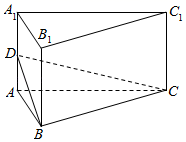
\includegraphics[width=36.0mm]{figs/image22.png}}\par\vspace{-1.0mm}\penalty10000

\zhankong{8mm}

\begin{ansblock}[导-章末-高考1]
% ans:导-章末-高考1
\ansnote{高考1}{\(P\) 为 \(CC_{1}\) 中点（答案不唯一，开放条件填充）}
\end{ansblock}

\liB{高考\textbf{2}}{中档(1.1.3)}{如图，在棱长为2的正方体\(ABCD\text{-}\penalty100 A_{1}B_{1}C_{1}D_{1}\)中，点\(E\)为棱\(CD\)的中点，点\(F\)为底面\(ABCD\)内一点，给出下列三个论断：}{}

\bindp {\fontsize{10.5pt}{19pt}\selectfont ①\(A_{1}F\perp BE\)；\qquad ②\(A_{1}F=3\)；\qquad ③\(S_{\triangle ADF}=2S_{\triangle ABF}\).\par}

\bindp {\fontsize{10.5pt}{19pt}\selectfont 以其中的一个论断作为条件，另一个论断作为结论，写出一个正确的命题：\kongbai{}.（注：论断②不能作条件也不能作结论.）}

\bindp \par\vspace{1.9mm}\penalty10000\noindent\makebox[\linewidth][c]{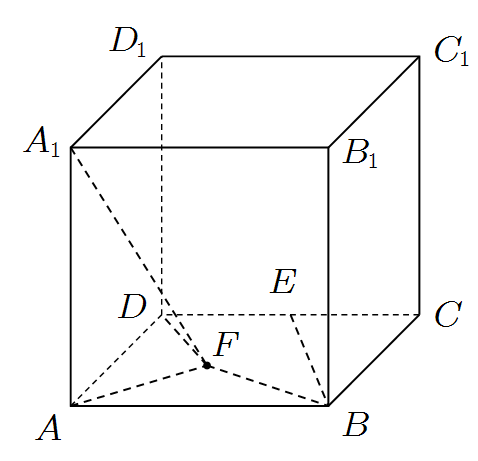
\includegraphics[width=40.0mm]{figs/image24.png}}\par\vspace{-1.0mm}\penalty10000

\begin{ansblock}[导-章末-高考2]
% ans:导-章末-高考2
\ansnote{高考2}{①\(\Leftrightarrow\)③（①作条件③作结论、③\(\Rightarrow\)①亦可；②不能作条件也不能作结论）}
\end{ansblock}

\columnbreak

\liB{高考\textbf{3}}{中档(1.2.3)}{如图，在三棱柱\(ABC\text{-}\penalty100 A_{1}B_{1}C_{1}\)中，侧面\(BCC_{1}B_{1}\)为正方形，平面\(BCC_{1}B_{1}\perp\)平面\(ABB_{1}A_{1}\)，\(AB=BC=2\)，\(M,N\)分别为\(A_{1}B_{1},AC\)的中点.}{}

\bindp {\fontsize{10.5pt}{19pt}\selectfont (1)求证：\(MN\parallel\)平面\(BCC_{1}B_{1}\)；\par}

\bindp {\fontsize{10.5pt}{19pt}\selectfont (2)再从条件①、条件②这两个条件中选择一个作为已知，求直线\(AB\)与平面\(BMN\)所成角的正弦值.\par}

\bindp {\fontsize{10.5pt}{19pt}\selectfont 条件①：\(AB\perp MN\)；条件②：\(BM=MN\).\par}

\bindp {\fontsize{10.5pt}{19pt}\selectfont 注：如果选择条件①和条件②分别解答，按第一个解答计分.\par}

\bindp \par\vspace{1.9mm}\penalty10000\noindent\makebox[\linewidth][c]{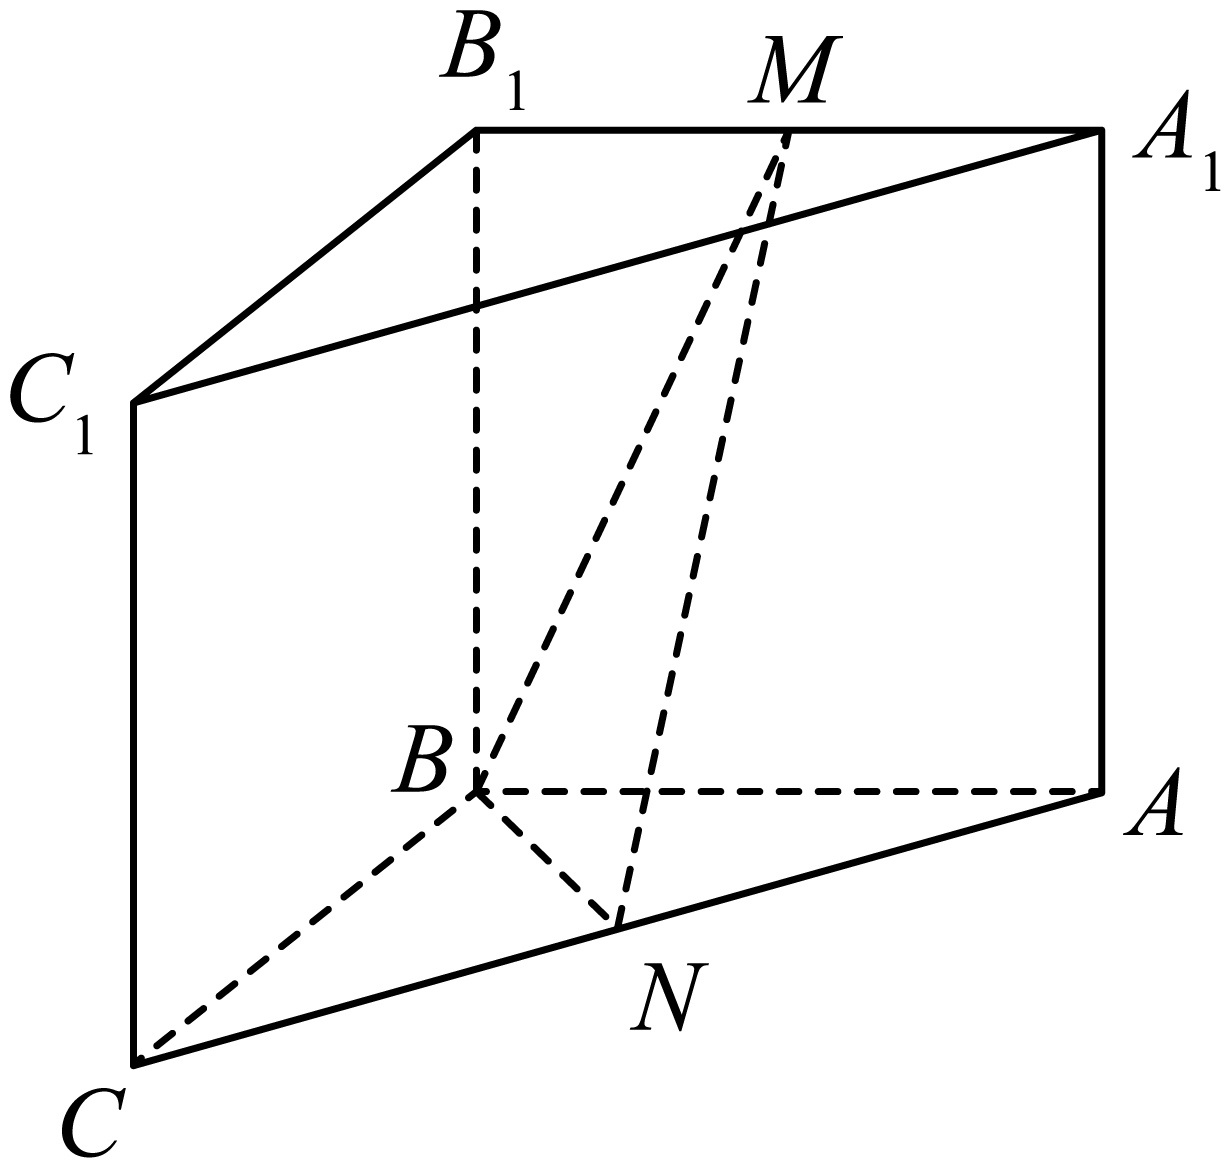
\includegraphics[width=44.0mm]{figs/image33.png}}\par\vspace{-1.0mm}\penalty10000

\zhankong{6mm}

\begin{ansblock}[导-章末-高考3]
% ans:导-章末-高考3
\ansnote{高考3}{(1)证明见解析；(2)\(\dfrac{2}{3}\)（①②两路同值）}
\end{ansblock}

\liB{高考\textbf{4}}{中档(1.2.4)}{如图，在四棱锥\(P\text{-}\penalty100 ABCD\)中，底面\(ABCD\)是边长为2的菱形，\(\angle ABC=60^\circ\)，\(\triangle PAB\)为正三角形，且侧面\(PAB\perp\)底面\(ABCD\)，\(E\)为线段\(AB\)的中点，\(M\)在线段\(PD\)上.}{}

\bindp {\fontsize{10.5pt}{19pt}\selectfont (1)求证：\(PE\perp AC\)；\par}

\bindp {\fontsize{10.5pt}{19pt}\selectfont (2)是否存在点\(M\)，使二面角\(M\text{-}\penalty100 EC\text{-}\penalty100 D\)的大小为\(60^\circ\)，若存在，求出\(PM/PD\)的值；若不存在，请说明理由.\par}

\bindp \par\vspace{1.9mm}\penalty10000\noindent\makebox[\linewidth][c]{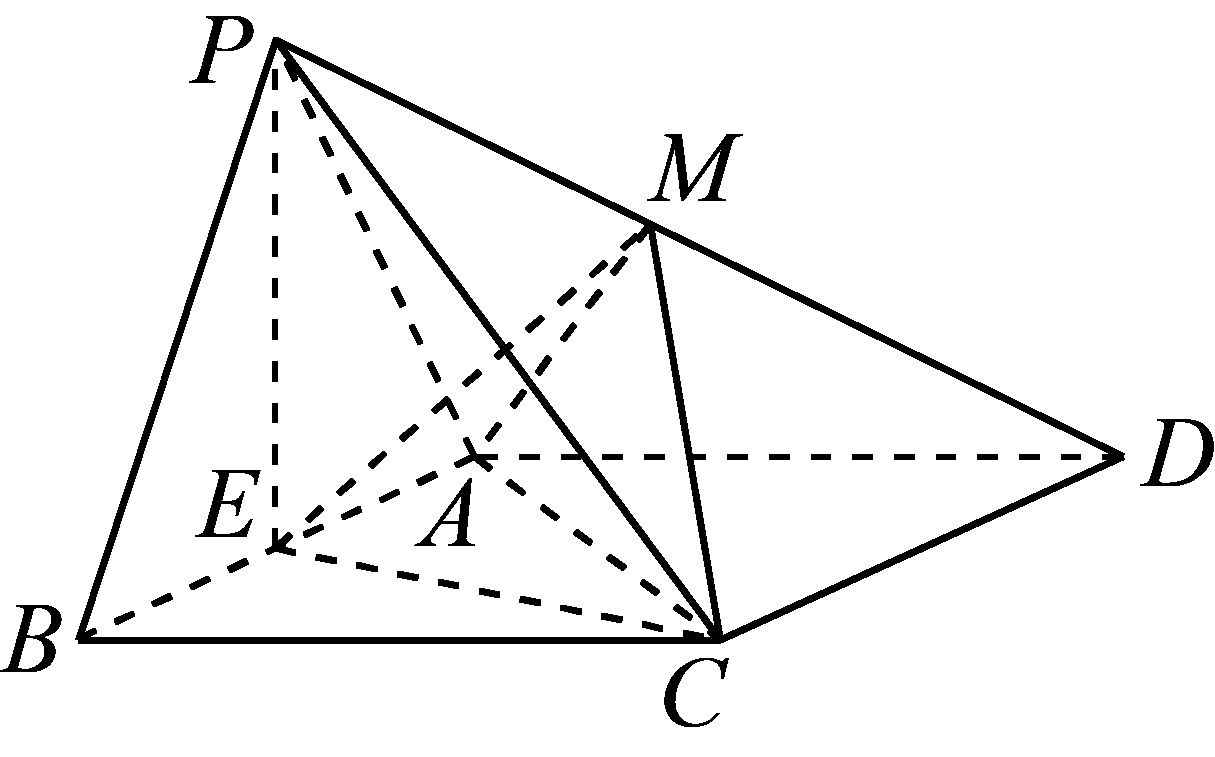
\includegraphics[width=50.0mm]{figs/image47.png}}\par\vspace{-1.0mm}\penalty10000

\begin{ansblock}[导-章末-高考4]
% ans:导-章末-高考4
\ansnote{高考4}{(1)证明见解析；(2)存在，\(\dfrac{PM}{PD}=\dfrac{1}{3}\)}
\end{ansblock}

\end{multicols}

\clearpage

% ============================================================
% 板块三·知识脉络（全章结构文本树；节名＝时间线基准表口径；全品原章末脉络图不在手＝文本树代偿登记）
% ============================================================
\begin{multicols}{2}
\emergencystretch=1em

\huaxing{知}{识}{脉}{络}{全章结构\quad 主线贯通}

\par\glueguard{2}\addvspace{2pt}%
\noindent\anlabel{[知识脉络]}\hspace{0.5em}{\fangsong 本章以“向量化”贯通立体几何：先用向量刻画空间元素，再把位置关系与角、距离全部转化为向量运算．}\par\addvspace{3pt}

\bindp {\fontsize{10.5pt}{19pt}\selectfont 第1章\quad 空间向量与立体几何\par}

\bindp {\fontsize{10.5pt}{19pt}\selectfont ┣ 1.1\quad 空间向量及其运算\par}

\bindp {\fontsize{10.5pt}{19pt}\selectfont ┃\qquad ┣ 1.1.1\quad 空间向量及其运算：概念与线性运算、数量积与夹角、投影向量\par}

\bindp {\fontsize{10.5pt}{19pt}\selectfont ┃\qquad ┣ 1.1.2\quad 空间向量基本定理：共面向量定理、基底与分解\par}

\bindp {\fontsize{10.5pt}{19pt}\selectfont ┃\qquad ┗ 1.1.3\quad 空间向量的坐标与空间直角坐标系：坐标运算、模与夹角公式\par}

\bindp {\fontsize{10.5pt}{19pt}\selectfont ┗ 1.2\quad 空间向量在立体几何中的应用\par}

\bindp {\fontsize{10.5pt}{19pt}\selectfont \qquad ┣ 1.2.1\quad 空间中的点、直线与空间向量：方向向量、线线角\par}

\bindp {\fontsize{10.5pt}{19pt}\selectfont \qquad ┣ 1.2.2\quad 空间中的平面与空间向量：法向量、平行与垂直的判定\par}

\bindp {\fontsize{10.5pt}{19pt}\selectfont \qquad ┣ 1.2.3\quad 直线与平面的夹角\par}

\bindp {\fontsize{10.5pt}{19pt}\selectfont \qquad ┣ 1.2.4\quad 二面角\par}

\bindp {\fontsize{10.5pt}{19pt}\selectfont \qquad ┗ 1.2.5\quad 空间中的距离：点线距、点面距、线面距、面面距\par}

\zhankong{4mm}

\par\glueguard{2}\addvspace{2pt}%
\noindent\anlabel{[方法主线]}\hspace{0.5em}设(选基底或建系)→表(点与向量坐标化)→算(套用坐标公式)→判(由运算结果判定位置关系、求出角与距离).\par\addvspace{3pt}

\bindp {\fangsong 使用提示：回看上方题型归类，按“设→表→算→判”四步复盘每型例题，标明自己卡在哪一步，再针对性重做该型的变式题.}

\end{multicols}

\tailfill
\end{document}
